\chapter{A Third Target: Playing and Debugging with PRG32-QT}
\label{ch:qt}

The two targets of Chapter~\ref{ch:firstbuild} run your code \emph{natively}: on
the ESP32\nobreakdash-C6 itself, or on Espressif's QEMU model of a sibling chip.
This chapter introduces a third way to run a cartridge, and it is different in
kind. \textbf{PRG32-QT} is a desktop, mobile, and television application that
reads a portable \fname{.prg32} file and \emph{interprets} its \riscv
instructions one at a time \citep{prg32qt}. Because it executes each instruction
itself, it can do something neither native target can do comfortably: stop
between any two instructions and show you every register. For a course about
computer architecture, that is a microscope.

\section{Three ways to run one cartridge}

It helps to have the three targets side by side before choosing one for a task.

\begin{center}
\begin{tabularx}{\linewidth}{@{}lXXX@{}}
\toprule
 & ESP32-C6 board & Espressif QEMU & PRG32-QT \\
\midrule
How code runs & natively on the chip & natively on an emulated ESP32-C3 &
  interpreted RV32IMAC guest \\
Needs ESP-IDF & yes & yes & no (to play) \\
Cartridge arrives by & Wi-Fi upload, Store & staging into flash image &
  file import, Store, HTTP upload \\
Sound & I2S amplifier & host audio over UART & host audio \\
Instruction stepping & with JTAG and GDB & with GDB & built-in debugger \\
Runs on & the kit & Windows, Linux, macOS & desktop, Raspberry Pi, iOS,
  Android, TV \\
\bottomrule
\end{tabularx}
\captionof{table}{The three hosts of a \prg cartridge. The cartridge file is the
same in every column.}
\label{tab:threehosts}
\end{center}

\begin{prgconcept}
A \emph{portable} cartridge does not contain the addresses of the firmware it
will meet. It calls the runtime through a numbered table, the cartridge ABI, and
any host that provides that table can run it. The board's firmware is one such
host; QEMU running the same firmware is a second; PRG32-QT, which implements the
table in C++, is a third.
\end{prgconcept}

The preface said that \prg ``is deliberately not a CPU emulator,'' and that
remains true of the platform's reference targets: the measurements of
Appendix~\ref{app:perf} are taken on real silicon. PRG32-QT does not replace
that; it complements it. Use the board when you want the truth about time, and
PRG32-QT when you want the truth about a register.

\section{Installing and first run}

Students who only want to \emph{play and debug} do not need a compiler at all:
each PRG32-QT release publishes installers for Windows, macOS (Apple Silicon and
Intel), Linux, and Raspberry Pi OS, an Android package, and builds for iOS and
television devices \citep{prg32qt}. On first launch the application shows the
same Setup screen the firmware shows, pointed at the public Cartridge Store. From
there you can browse the catalogue, download a cartridge, and run it, or import a
\fname{.prg32} file you built yourself.

\begin{center}
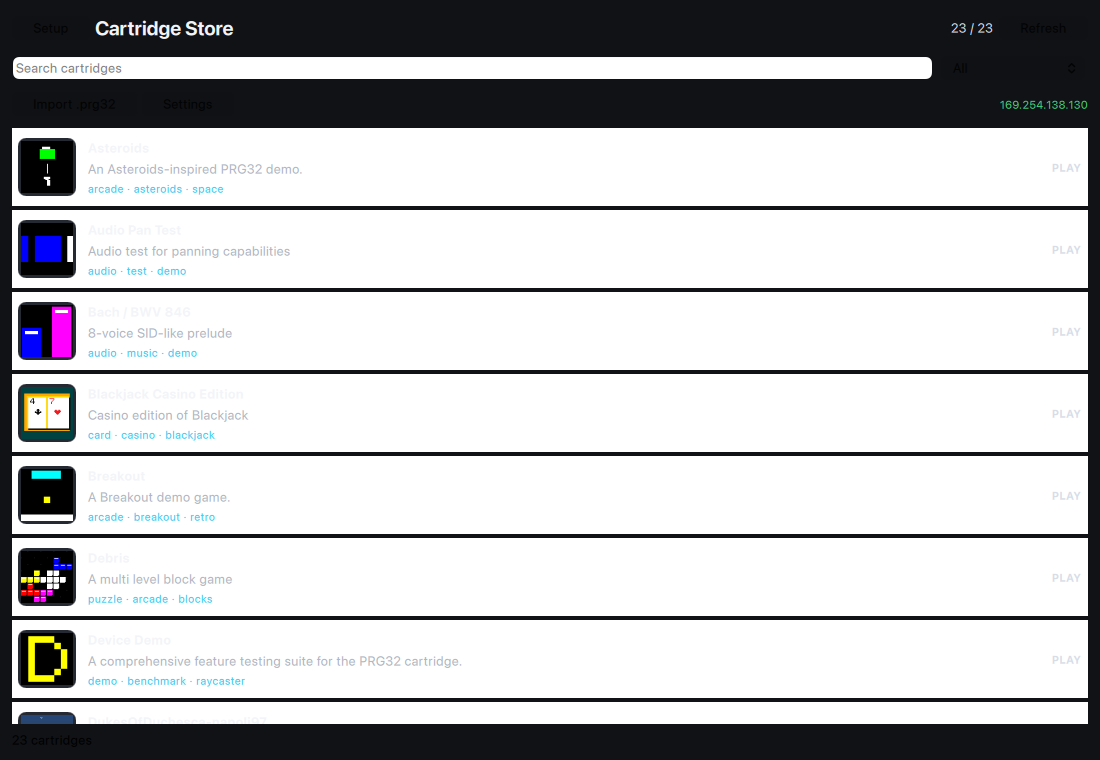
\includegraphics[width=0.78\linewidth]{figures/prg32qt-store.png}
\captionof{figure}{The Cartridge Store browser inside PRG32-QT. Downloads are
architecture-aware: the application asks the Store for a variant it can run
\citep{prg32qt}.}
\label{fig:qtstore}
\end{center}

The controls mirror the kit. On a keyboard the arrow keys (or
\kbtn{W}\,\kbtn{A}\,\kbtn{S}\,\kbtn{D}) are the joystick, \kbtn{Z} or \kbtn{J} is
button~A, \kbtn{X} or \kbtn{K} is button~B, and \kbtn{Enter} or \kbtn{Space} is
Start/Select. A USB or Bluetooth game controller is recognised when it is plugged
in; phones and tablets show touch controls instead.

Students who want to study the host itself can build its Qt-free core, which
contains the cartridge parser, the RV32IMAC interpreter, and the ABI
implementation, and run its test suite without installing Qt at all.

\lstinputlisting[style=bash,
  caption={Building and testing the portable runtime core of PRG32-QT.}
]{scripts/prg32qt/build_core.sh}

\section{Three performance profiles}

An interpreter on a laptop is far faster than a 160\,MHz microcontroller, so a
cartridge that is comfortable in PRG32-QT might crawl on the board. To keep
students honest, the application offers three profiles in its Settings.

\begin{center}
\begin{tabularx}{\linewidth}{@{}lX@{}}
\toprule
Profile & Behaviour \\
\midrule
Accurate (default) & charges each instruction class and each ABI call a
  deterministic cost at the reference 160\,MHz clock and 33\,ms frame cadence;
  reports frames that would have been late on the board \\
Optimal & paces the game at 30 frames per second \\
Unlimited & runs as fast as the host allows \\
\bottomrule
\end{tabularx}
\captionof{table}{PRG32-QT performance profiles \citep{prg32qt}.}
\end{center}

\begin{prgwarn}
Accurate mode is a \emph{model}, not a measurement. It reproduces behaviour that
is visible to a portable cartridge; it is not a cycle-exact simulation of the
ESP32\nobreakdash-C6. Treat its ``late frame'' counter as an early warning, and
confirm any performance claim on real hardware with the method of
Appendix~\ref{app:perf}.
\end{prgwarn}

\section{The debugger: a microscope for the frame loop}

Open Settings, enable \emph{Run cartridges in RISC-V debug mode}, and run a
cartridge. The player stays on the left and remains playable; on the right a
panel shows the disassembled cartridge, the thirty-two integer registers, and a
window onto guest memory.

\begin{center}
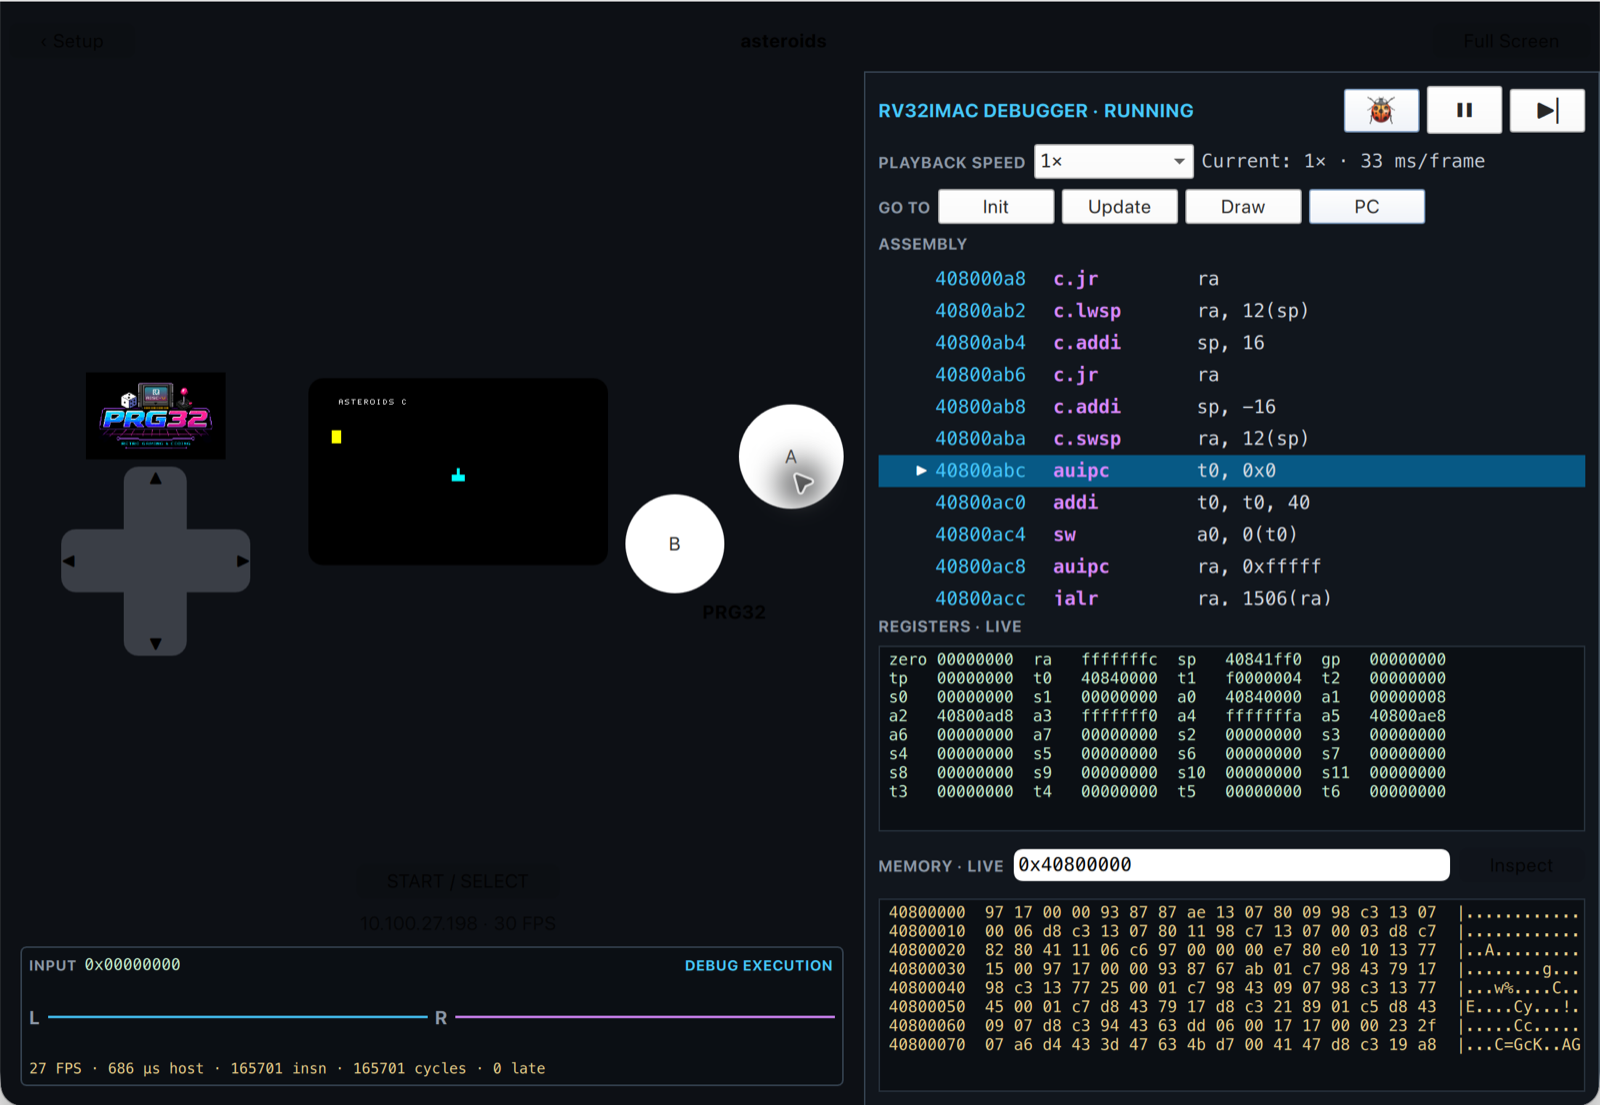
\includegraphics[width=\linewidth]{figures/prg32qt-debugger.png}
\captionof{figure}{The PRG32-QT debugger: the running game, the live assembly
listing with the next instruction highlighted, the registers, and a memory dump
\citep{prg32qt}.}
\label{fig:qtdebugger}
\end{center}

\begin{center}
\begin{tabularx}{\linewidth}{@{}lX@{}}
\toprule
Control & What it does \\
\midrule
Pause / Resume & stop and continue the cartridge; game input is frozen while
  paused \\
Step & execute exactly the highlighted instruction and stay paused \\
Speed & slow motion or fast forward, from $0.01\times$ to $4\times$ \\
Init / Update / Draw & jump the listing to that entry point without executing
  anything \\
PC & follow the live program counter \\
Gutter click & set or clear a breakpoint on that instruction \\
Memory address & show 128 bytes of guest memory in hexadecimal and ASCII \\
\bottomrule
\end{tabularx}
\captionof{table}{The debugger controls.}
\label{tab:qtdebug}
\end{center}

Everything the assembly track asks you to imagine becomes something you can
watch. Chapter~\ref{ch:asm1} says that \code{call} writes the return address into
\reg{ra}; step over a \code{call} and see \reg{ra} change. Chapter~\ref{ch:asm2}
says the input bitmask arrives in \reg{a0}; set a breakpoint after
\code{call prg32\_input\_read}, hold the left arrow, resume, and read
\code{0x00000001} in \reg{a0}. The cartridge is loaded at address
\code{0x40800000}, so a variable declared in \code{.data} can be found by typing
its address into the memory field and watching the bytes change as you play.

\begin{prgtry}
Build the complete C Pong of Appendix~\ref{app:worked} and import it into
PRG32-QT in debug mode. Select \textbf{Update}, set a breakpoint on its first
instruction, and resume. When execution stops, step until you pass the call to
\code{prg32\_input\_read}. Record \reg{a0} three times: with no key held, with
the left arrow held, and with left and \kbtn{Z} held together. Explain the three
values using Table~\ref{tab:buttons}.
\end{prgtry}

\begin{prgaside}
The home computers this book admires shipped with a ``monitor'': a tiny built-in
program that let the owner stop the machine, inspect memory, and change it by
hand. A generation of programmers learned how a processor works by pressing a
freeze button in the middle of a game. A debugger that pauses a running
cartridge and shows its registers is the same idea, forty years on.
\end{prgaside}

\section{Driving PRG32-QT from the toolchain}

While it runs, PRG32-QT announces itself on the local network as
\code{\_prg32.\_tcp.local.} and serves the same small HTTP interface as the
board, so the upload command you already know works against it. It adds one
route the constrained firmware does not have, \code{/api/debug}, and the \prg
tooling wraps that route in a \code{debug} command \citep{prg32repo,prg32qt}.

\lstinputlisting[style=bash,
  caption={Deploying a cartridge to a running PRG32-QT and controlling its
  debugger from a script.}
]{scripts/prg32qt/deploy_and_debug.sh}

This turns the debugger into a laboratory instrument. A script can pause a
cartridge, step a fixed number of instructions, read the registers as JSON, and
compare them with the values a student predicted on paper.

\begin{prgwarn}
The device API is meant for a trusted classroom network. It accepts uploads and
debugger commands from anyone who can reach the port. Do not expose it to the
open Internet.
\end{prgwarn}

\section{Choosing the right target}

A sensible working rhythm uses all three hosts. Develop and debug in PRG32-QT,
where a build takes seconds and a wrong branch can be watched as it is taken.
Confirm in QEMU, which runs the real firmware and therefore the real loader,
status bands, and setup menu. Finish on the board, where time, sound, and the
feel of the joystick are real.

\begin{prgcheck}
You are ready to continue when you can run a Store cartridge in PRG32-QT, import
one you built yourself, pause it, single-step an instruction, and say which
register changed. You should also be able to explain why a frame rate observed
in PRG32-QT is not evidence about the board.
\end{prgcheck}
